\section{Electric}

Kolejnym programem do projektowania schematów układów scalonych jest Electric,
opracowany przez S. M. Rubina w 1981 roku.
Od samego początku posiadał otwarty kod źródłowy
oraz był udostępniany wielu uczelniom na całym świecie.
Electric jest oficjalnym pakietem GNU, co oznacza,
że jest dystrybuowany jako wolne oprogramowanie zgodnie z zasadami projektu GNU~\cite{electric_gnu}.
Projekt ten jest inicjatywą, która ma na celu rozwój wolnego oprogramowania,
umożliwiającego swobodne korzystanie, modyfikowanie i rozpowszechnianie~\cite{gnu_site}.
Program Electric był oryginalnie napisany w języku C,
natomiast w 2003 rozpoczęto proces tłumaczenia na język Java, zakończony sukcesem w 2005 roku~\cite{electric_gnu}.
Dzięki temu program jest dostępny na każdym systemie,
na którym zainstalowana jest Java w wersji 1.6 lub nowszej.
Do samej instalacji wystarczy natomiast pobrać plik \texttt{.jar} z oficjalnej strony programu~\cite{electric_sfs}.
Podobnie jak Microwind, Electric jest oprogramowaniem EDA, zawierający wiele modułów wspierających projektowanie układów scalonych.
Większość nich jest pod postacią dodatkowo instalowanych wtyczek,
poszerzających jego funkcjonalność~\cite{electric_sfs, electric_gnu}.
Dzięki wykorzystaniu Javy, Electric posiada nowocześniejszy interfejs graficzny,
pokazany na rys.~\ref{fig:electric_okno}.

\begin{figure}[h]
    \centering
    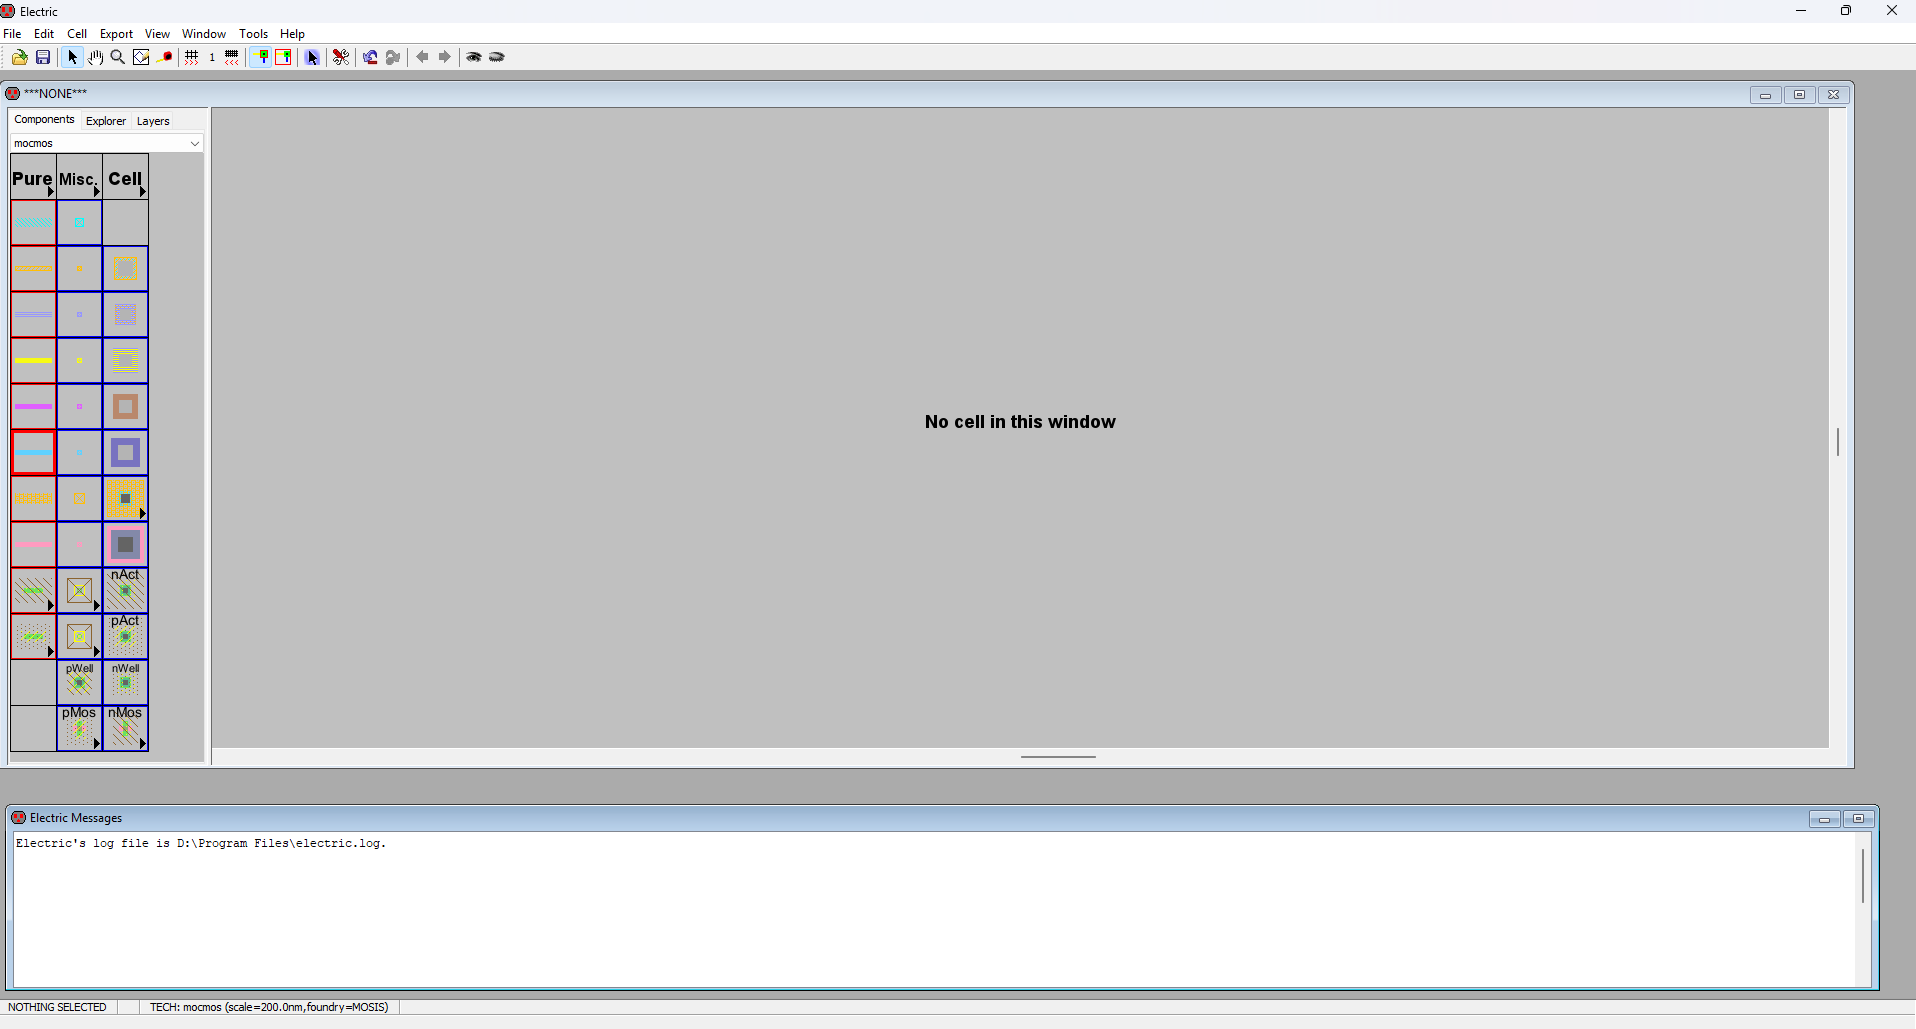
\includegraphics[width=.9\textwidth]{chapters/chapter2/img/electric_okno}
    \caption[Widok głównego okna programu Electric.]{Widok głównego okna programu Electric, źródło:~\cite{electric_sfs}.}
    \label{fig:electric_okno}
\end{figure}
%\indent Electric charakteryzuje się całkowicie odmienną metodą projektowania topografii niż większość programów.
\indent Electric stosuje metodę projektowania topografii odmienną od większości innych narzędzi tego typu.
Podobnie jak edytory schematów elektrycznych, opiera się na podejściu połączeniowym,
%w przeciwieństwie do reszty, gdzie występuje podejście geometryczne, czyli rysowanie prostokątów.
w odróżnieniu od większości edytorów topografii, które wykorzystują podejście geometryczne,
polegające na rysowaniu prostokątów.
Oparcie projektowania o metodę połączeń polega na wstawianiu gotowych elementów,
które pełnią funkcję węzłów, %będących węzłami,
a następnie łączeniu ich ze sobą, przy czym program sam dba o poprawne połączenia i wybór warstwy do tego.
%Na przykład tranzystor jest już gotowym elementem,
Przykładem gotowego elementu jest tranzystor,
który można wstawić od razu na schemat
i nie trzeba specjalnie rysować, jak to jest w przypadku programów Magic czy Microwind.
%Podejście to upraszcza znacząco proces projektowania oraz ułatwia analizę obwodu dzięki gotowym połączeniom,
Takie podejście znacząco upraszcza proces projektowania i ułatwia analizę obwodów dzięki gotowym połączeniom.
%natomiast może być to mniej efektywne w przypadku złożonych układów o nietypowych geometriach
Może jednak okazać się mniej efektywne w przypadku złożonych układów o nietypowych geometriach.
%oraz wymagać ponownej nauki dla osób przyzwyczajonych do innych programów,
Ponadto wymaga adaptacji ze względu na inny proces projektowania,
o czym wspomina sam autor programu~\cite{electric_computer_aids}.\\
%natomiast problem może stanowić tworzenie układów o bardziej skomplikowanej i złożonej geometrii.\\
Sposób poruszania się po obszarze roboczym oraz skróty klawiszowe są natomiast bardziej zgodne z obecnymi standardami,
dzięki czemu program staje się bardziej intuicyjny w obsłudze.
Przykładowo poruszanie się po obszarze roboczym odbywa się poprzez przytrzymanie środkowego przycisku myszy
i jednoczesne przesunięcie kursora.
Prócz stałych pasków narzędzi i menu, program opiera się na pływających oknach,
dzięki czemu można jednocześnie mieć wyświetlone kilka narzędzi jednocześnie.
Na rys.~\ref{fig:electric_okno} przedstawiono okno do edycji schematu oraz okno dziennika zdarzeń.
Edytor zamiast palety warstw posiada okno z dostępnymi elementami, połączeniami, węzłami połączeń
i kontaktami pomiędzy warstwami.
W przypadku Electrica, do przedstawiania warstw wykorzystuje się jednolite kolory, oraz wzory,
co przedstawiono na rys.~\ref{fig:electric_tran}.
Przy edycji oraz rysowaniu topografii można zauważyć miganie elementów,
co wskazuje, że cały widok jest na nowo renderowany po każdej edycji lub przesunięciu,
co przy większych projektach może być uciążliwe, a także mało wydajne.

\begin{figure}[h]
    \centering
    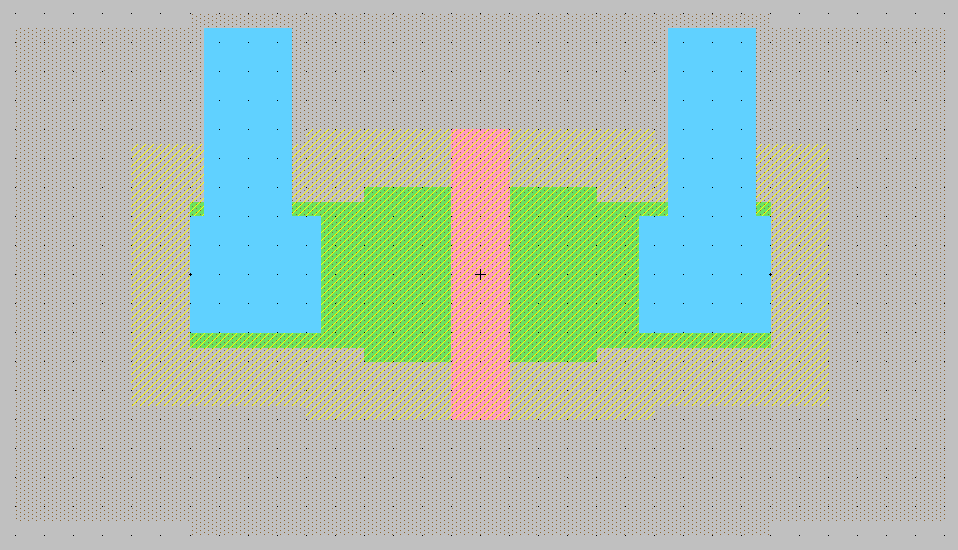
\includegraphics[width=.9\textwidth]{chapters/chapter2/img/electric_tran}
    \caption[Przykład tranzystora pMOS narysowanego w programie Electric]
    {
        Przykład tranzystora pMOS narysowanego w programie Electric,
        źródło: opracowanie własne.
    }
    \label{fig:electric_tran}
\end{figure}
